\section{Grand Canonical Monte Carlo Simulation}
\label{Chap:Mech:GCMC}

\subsection{Grand Canonical Ensemble}

The canonical ensemble is a statistical ensemble that consists of $N$ atoms and is in thermodynamic equilibrium with a big reservoir. Energy transfer is allowed between the system and the big reservoir, but particle transfer is impermissible. The big reservoir can be described as a system with relatively large heat capacity, and its temperature $T$ remains constant in spite of any energy transfer. Grand canonical ensemble is a statistical ensemble that can exchange particles with a reservoir as an open system. Besides, the big reservoir can also act as an infinite heat resource allowing heat transfer as shown in Fig. \ref{Chap:Meth:GCMC:fig1}. \cite{frenkel2001understanding} Therefore in the grand canonical ensemble, the number of atoms $N$ in the system can be changed and chemical potential of each element $\mu_i$, the volume of the system $V$ and temperature $T$ are fixed, hence this system as known as $\mu VT$ system.

\begingroup
\begin{figure}[!ht]
  \centering
  \subfigure[]{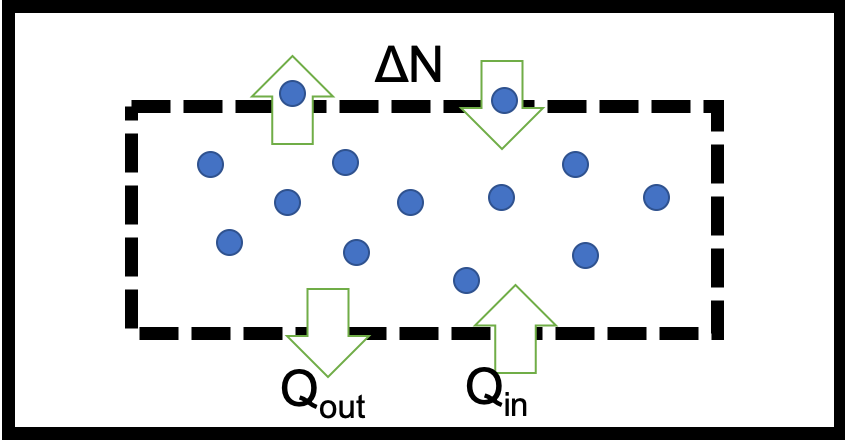
\includegraphics[width=0.85\linewidth]{Methods/plots/grand-canonical-ensemble.png}}
  \caption[Illustration plot of grand canonical ensemble]{Illustration plot of grand canonical ensemble. Black line shows the universe. Black dashed line confines the ensemble. Blue solid circles are atoms in the system.}
  \label{Chap:Meth:GCMC:fig1}
\end{figure}
\endgroup

\subsection{Monte Carlo Methods}
\label{Chap:Mech:GCMC:MC}

\ac{MC} methods are a broad class of computational algorithms that rely on repeated random sampling to obtain numerical results for a problem that is difficult to solve in principle. The physics behind is to use randomness to solve problems that might be deterministic. They are often used in mathematical \cite{hubbard2009modeling} and physical \cite{bortz1975new} problems. In this thesis, \ac{MC} methods are used to do optimization for complex \ac{GB} structures in Chap. \ref{Chap:Ag/ZnO:GB}, thin-film morphology in Chap. \ref{chap:Ag/ZnO} and solving stochastic time evolution in Chap. \ref{chap:Al/Vac}. A general \ac{MC} algorithm involves: i) drawing a random number $u \in (0,1]$ and ii) accepting/rejecting event base on Boltzmann probability.

\subsection{Grand Canonical Monte Carlo Simulation}
\label{Chap:Mech:GCMC:GCMC}

\ac{GCMC} simulation combines the grand canonical ensemble with \ac{MC} simulations. Following grand canonical($\mu VT$) ensemble discussed above, the number of atoms $N$ in the ensemble can be changed, thus grants two types of events, inserting a new atom and deleting an existing atom. In addition to these two events, moving an atom to a different location is also considered in the event list. Therefore, the probability of accepting moving an existing atom is via \cite{frenkel2001understanding}:
\begin{align}
acc(s \rightarrow s') = \text{min}(1, exp(-\beta(U(s'^N) - U(s^N))
\label{Chap:Meth:eq:acc:move}
\end{align}
inserting a new atom:
\begin{align}
acc(N \rightarrow N+1) = \text{min}(1, \frac{V}{\wedge^3(N+1)}exp(\beta(\mu - U(N + 1) + U(N)))) \label{Chap:Meth:eq:acc:insert}
\end{align}
and removing an exiting atom:
\begin{align}
acc(N \rightarrow N-1) = \text{min}(1, \frac{\wedge^3(N)}{V}exp(-\beta(\mu + U(N - 1) - U(N)))) \label{Chap:Meth:eq:acc:remove}
\end{align}
where, $\beta$ is the thermodynamic beta and $\wedge$ is the de Broglie wavelength. Additionally, \ac{MD} steps are usually combined together with \ac{GCMC} simulations to reduce the thermal instability or stress introduced by randomly inserting and moving atoms, as know as the hybird \ac{MC}/\ac{MD} method in Chap. 4.4 of Frenkel 2001 \cite{frenkel2001understanding}.